\section{Previous Work}

Using machine learning for condition monitoring is not new.
There are typically three approaches:
\begin{enumerate}
	\item Supervised algorithms using sensor data and maintenance data.
    \item Unsupervised algorithms using only sensor data.
    \item Semi-supervised algorithms using only \textit{healthy} sensor data.
\end{enumerate}

% supervised
Supervised methods require labelled data.
Labelling is the process of associating an output with a set of variable values at a certain point in time.
For example, if there is knowledge to when the failures occurred and there are sufficient failures, the data can be labelled as healthy or not.
Unfortunately, there is just not enough failure data in practice to make this feasible.
Instead, failure data can be estimated and artificially generated \cite{Sotiris2010AnomalyDT}.
But even then the algorithms are limited to a binary outputs.

Using $k$-nearest neighbours (kNN) to estimate asset condition directly is difficult due to noise, and requires domain specific knowledge to choose appropriate variables.
One paper improves on kNN methods for detecting the levels of severity for cracks in gears \cite{lei2009gear}.
The disadvantage in these approaches is that it requires significant data in a variety of conditions, and it uses classification to identify a severity level instead of a numerical value.

Researchers in \cite{opt} train an autoencoder on healthy imaging data to get a feature representation in a smaller number of dimensions.
Utilizing the Support Vector Machine (SVM), they learn a decision boundary to identify anomalies.
This approach is interesting for high dimensional data but focuses on point anomalies, where as we are interested in projecting asset health over time.

% self organized maps
A Self-Organizing Map (SOM) is a type of neural network that is often used as a dimensionality reduction technique as it produces a low dimensional representation of the training samples \cite{map1990self}.
The two most relevant papers on using SOMs for condition maintenance were used on aircraft engines and ball bearings \cite{come2010aircraft} \cite{Tian2014AnomalyDU}.
The SOM can be visualized directly as a tool to identify failures as in Figure \ref{aircraft}, where data points 517-607 are clearly anomalous.
\begin{figure}[!h]
    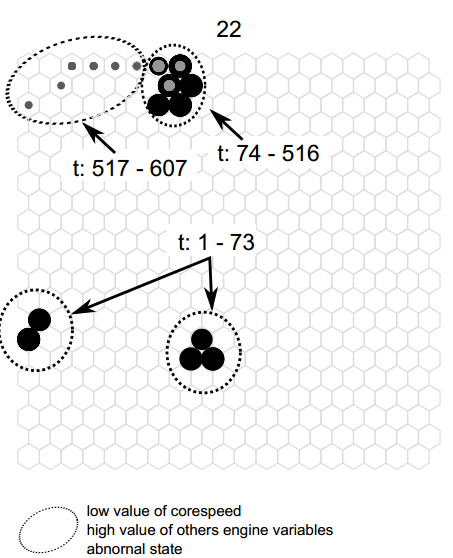
\includegraphics[scale=0.5]{aircraft}
    \centering
    \caption{SOM map being used to identify anomalous behaviour \cite{come2010aircraft}.}
    \label{aircraft}
\end{figure}
%Training a SOM on healthy asset data, researchers were able to output a health indication in an interpretable way but still lacked a quantifiable measure \cite{5524339}.
Alternatively, Huang et al. were able to use the minimum quantization error between a test point and the closest neuron of the SOM as the health indicator for ball bearings \cite{som-1}.
% Math equation/formula
\begin{equation}
	Q = \min_{k} \Vert D-B_k \Vert
\end{equation}
 Where $Q$ is the minimum quantization error, $D$ is a test set observation, and $B_k$ is the weight vector of the $k^{th}$ closest neuron of the SOM.
But, using quantization error can be improved as it is sensitive to noise.
Researchers Tian et al. use a SOM and a $k$-nearest neighbours algorithm (see Figure \ref{knn}) in combination with the Euclidean distance between the test data and the healthy data to develop a more robust health score.
\begin{figure}[!h]
    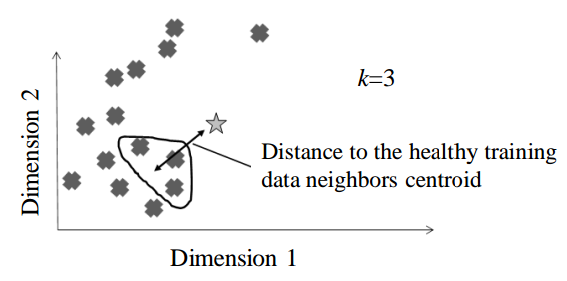
\includegraphics[width=8cm]{knn}
    \centering
    \caption{A health score can be used as the distance from a test point to a cluster (or a neuron in a SOM) \cite{Tian2014AnomalyDU}.}
    \label{knn}
\end{figure}
